\documentclass[letterpaper, 10 pt]{IEEEconf}

\usepackage{amsmath}
\usepackage{graphicx}
\usepackage{booktabs}
\usepackage{array}
\usepackage{url}

\title{\LARGE \bf
Lightweight Wheel-Candidate Filtering for Virtual Wheel Try-On
}

\author{
Egor Kuznetsov and Nikolai Lutsenko%
\thanks{The authors are with Skolkovo Institute of Science and Technology.
This report describes a course project for a deep learning project work.}
}

\begin{document}

\maketitle
\thispagestyle{empty}
\pagestyle{empty}

\begin{abstract}
This project studies a lightweight supervised classifier for filtering wheel
candidate crops before an expensive virtual wheel try-on stage. The model
receives a candidate crop and predicts whether it is a usable wheel candidate
or an invalid false positive. The goal is not full wheel detection on complete
vehicle images, but a focused second-stage decision that can reduce unnecessary
downstream visual-language or image-generation calls. We build a cleaned binary
dataset from open-source vehicle images using a custom PyQt annotation tool,
obtain 1,767 crop samples from 586 source images, create leakage-safe grouped
train, validation, and test splits, implement a classical baseline, and fine-
tune compact pretrained CNN backbones. The final MobileNetV3-Large model
achieves 0.868 accuracy, 0.828 valid-class precision, 0.933 valid-class recall,
0.877 valid-class F1, and 0.947 ROC-AUC on the held-out test set. The remaining
errors are mostly caused by ambiguous invalid crops and visually difficult
wheel crops such as dark, blurred, occluded, or poorly localized candidates.
\end{abstract}

\section{Introduction}

Virtual wheel try-on systems commonly involve several processing stages. A user
provides a vehicle image and a target wheel or rim image, and downstream models
produce an edited visualization. In such a pipeline, proposed wheel regions
must be checked before more expensive components are called. Some candidate
regions contain real and usable wheels. Others are false positives: background
patches, vehicle body parts, reflections, partial structures, or badly localized
wheel-like crops.

This project addresses this narrow filtering problem. Given a crop $x$, the
model predicts a binary label:
\begin{equation}
    f(x) \rightarrow y,\qquad y \in \{0,1\},
\end{equation}
where $y=1$ denotes a valid wheel candidate and $y=0$ denotes an invalid
candidate. The task is deliberately scoped as candidate filtering, not as full
object detection. A complete product pipeline would still require a detector or
candidate generator before this classifier.

The practical motivation is efficiency and robustness. A small local classifier
can remove many poor candidates before they reach expensive visual-language or
image-generation models. For this use case, false negatives are especially
important: rejecting a real wheel candidate can break the downstream try-on
workflow. False positives also matter because they waste computation, but they
are usually less damaging than missing a real wheel.

\section{Dataset}

\subsection{Source Data and Labels}

The dataset was derived from full-vehicle images downloaded from an open-source
vehicle/wheel detection image collection. We did not label whole images as
``contains a wheel'' or ``does not contain a wheel''. Instead, we converted the
raw vehicle images into a crop-level binary dataset. Each exported sample is a
specific candidate region with one of two labels:
\begin{itemize}
    \item \texttt{valid\_wheel\_candidate}: a visible and sufficiently localized
    wheel candidate;
    \item \texttt{invalid\_candidate}: a crop that is not suitable for further
    wheel try-on processing.
\end{itemize}

The final cleaned dataset combines two labeled crop exports. It contains 1,767
samples. The class distribution is nearly balanced: 884 valid candidates and
883 invalid candidates. The samples come from 586 unique source images.

\subsection{Annotation Tool and Workflow}

To create the crop-level labels within the project time budget, we implemented
a custom annotation tool in Python using PyQt6 and Pillow. The tool was used
for fast manual review over approximately one week. It opens a folder of raw
vehicle images, imports Pascal VOC XML boxes when they are available, allows the
annotator to draw or correct bounding boxes, and assigns a candidate label to
each box.

The tool was designed around the actual downstream task. It stores rich per-
image and per-object metadata, but the training target remains a simple binary
crop label. Image-level fields include vehicle type, viewpoint, image quality,
source type, and notes. Object-level fields include bounding-box coordinates,
object label, candidate label, binary label, wheel position, side, visibility,
crop quality, annotation source, and notes. The GUI also provides productivity
features such as progress filtering, search, automatic saving, keyboard
shortcuts for valid/invalid labels, zooming, panning, and one-click export of
all labeled crops.

The export step creates two class folders,
\texttt{valid\_wheel\_candidate/} and \texttt{invalid\_candidate/}, plus a
\texttt{labels.csv} file. The CSV records the crop path, binary label, source
image, original bounding box, expanded crop coordinates, and metadata. Crops are
exported with a configurable margin around the annotated box; the default tool
setting was 15\%.

\subsection{Train, Validation, and Test Split}

The split was constructed by grouping on \texttt{source\_relative\_path}. This
prevents crops from the same original image from appearing in different splits,
which is important because several candidate crops can come from one vehicle
image. The final leakage check reports a maximum of one split per source-image
group.

\begin{table}[t]
\caption{Leakage-safe grouped split summary.}
\label{tab:split}
\centering
\begin{tabular}{lrrrr}
\toprule
Split & Samples & Valid & Invalid & Sources \\
\midrule
Train & 1228 & 615 & 613 & 410 \\
Validation & 273 & 135 & 138 & 88 \\
Test & 266 & 134 & 132 & 88 \\
\bottomrule
\end{tabular}
\end{table}

\section{Method}

\subsection{Preprocessing}

All crops are converted to RGB, padded to a square aspect ratio, resized to
$224 \times 224$, and normalized with ImageNet statistics. Square padding is
used instead of direct non-uniform resizing to preserve the visual geometry of
the wheel candidate.

During training, moderate augmentations are applied: mild random resized crop,
horizontal flipping, small rotations, color jitter, and occasional Gaussian
blur. These transformations are intended to improve robustness to lighting,
viewpoint, and localization variability without changing the semantic label.

\subsection{Models}

The experiments compare a classical baseline with compact pretrained CNN
backbones:
\begin{itemize}
    \item a majority-class sanity baseline;
    \item logistic regression on simple image features;
    \item MobileNetV3-Large fine-tuned for binary classification;
    \item EfficientNet-B0 fine-tuned for binary classification.
\end{itemize}

MobileNetV3 and EfficientNet are appropriate choices for this problem because
they are compact enough for practical filtering while still benefiting from
ImageNet pretraining.

\subsection{Training Setup}

The deep models are trained with weighted cross-entropy, AdamW, cosine learning
rate scheduling, and early stopping. The class weights are kept balanced,
although the final cleaned dataset is already close to class-balanced. Mixed
precision is enabled when CUDA is available.

The decision threshold is selected on the validation set, not on the test set.
Because valid-wheel recall is the main product-oriented requirement, the
threshold search prefers thresholds that reach at least 0.90 validation recall
for the valid class, and then optimizes F1 and precision within that constraint.

\section{Results}

\subsection{Main Test Metrics}

Table~\ref{tab:results} reports held-out test metrics. The deep models
substantially outperform the classical baseline. MobileNetV3-Large gives the
best valid-class F1 score and the lowest false-negative count. EfficientNet-B0
has slightly higher ROC-AUC and PR-AUC, but it misses more true valid wheel
candidates at its selected operating threshold.

\begin{table*}[t]
\caption{Held-out test results. Precision, recall, and F1 are reported for the
valid-wheel class. Thresholds are selected on validation data.}
\label{tab:results}
\centering
\small
\begin{tabular}{lrrrrrrrrrrr}
\toprule
Model & Thr. & Acc. & Prec. & Recall & F1 & ROC-AUC & PR-AUC & TN & FP & FN & TP \\
\midrule
Sklearn baseline & 0.125 & 0.669 & 0.646 & 0.761 & 0.699 & 0.702 & 0.715 & 76 & 56 & 32 & 102 \\
MobileNetV3-Large & 0.460 & 0.868 & 0.828 & 0.933 & 0.877 & 0.947 & 0.948 & 106 & 26 & 9 & 125 \\
EfficientNet-B0 & 0.405 & 0.865 & 0.836 & 0.910 & 0.871 & 0.950 & 0.951 & 108 & 24 & 12 & 122 \\
\bottomrule
\end{tabular}
\end{table*}

The improvement over the baseline is large enough to show that transfer
learning is useful for this crop-filtering task. Compared with the logistic
regression baseline, MobileNetV3-Large increases valid-class F1 from 0.699 to
0.877 and reduces false negatives from 32 to 9.

\subsection{Training Dynamics}

Both deep models reach their best validation performance early. MobileNetV3-
Large obtains its best checkpoint at epoch 2. EfficientNet-B0 also obtains its
best checkpoint at epoch 2. After that point, training loss continues to fall,
while validation loss starts to increase. This indicates mild overfitting, which
is expected for a small and visually ambiguous dataset. Early stopping therefore
plays an important role in selecting a generalizable checkpoint.

\begin{figure}[t]
\centering
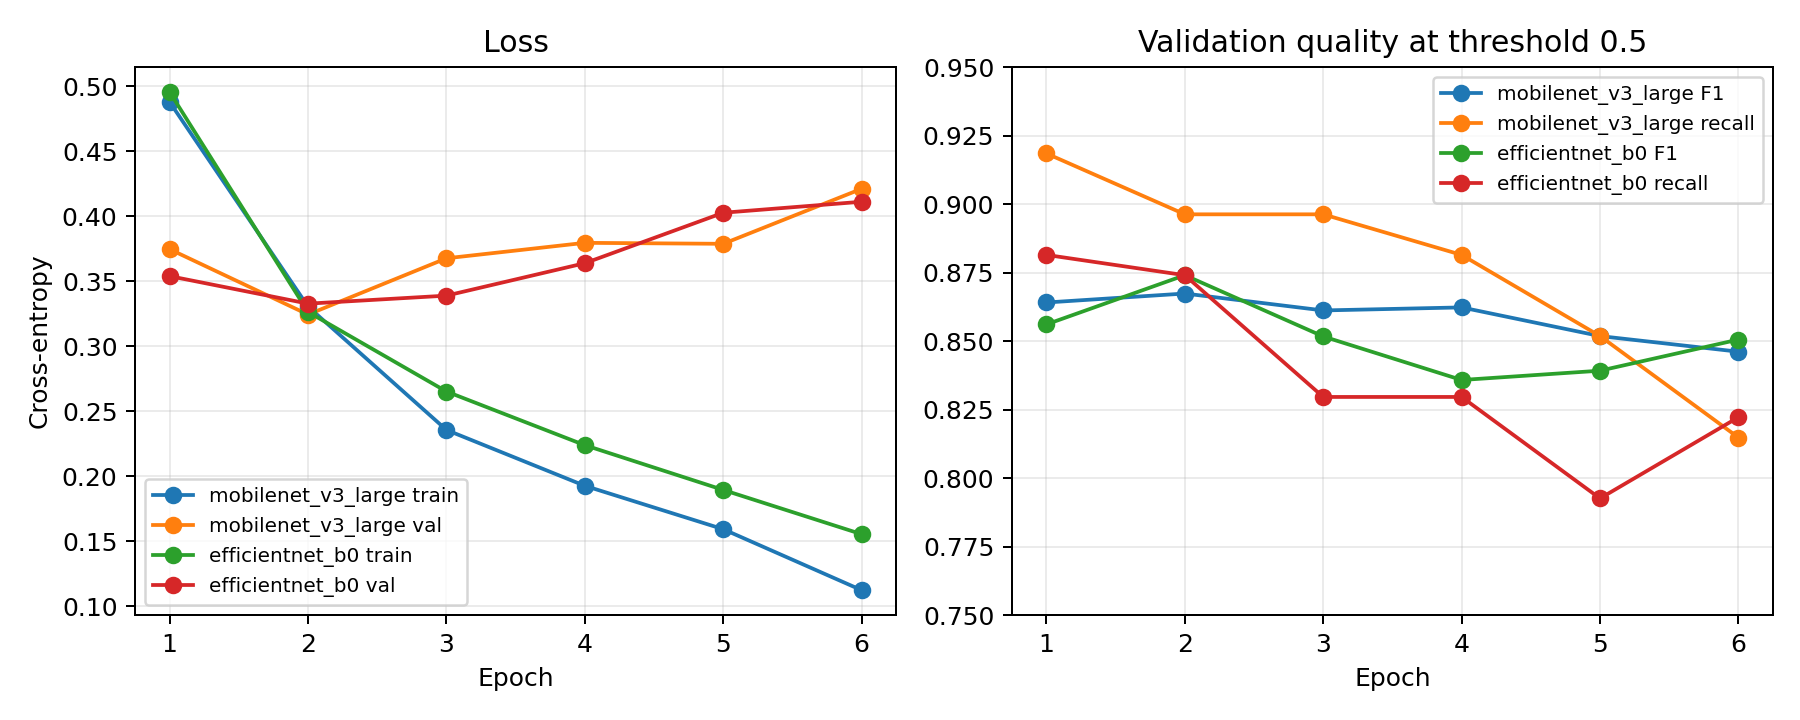
\includegraphics[width=\linewidth]{reports/training_history.png}
\caption{Training loss, validation loss, validation F1, and validation recall
for the two fine-tuned CNN models.}
\label{fig:history}
\end{figure}

\subsection{Confusion Matrix and Curves}

The confusion matrix of the selected MobileNetV3-Large model is shown in
Fig.~\ref{fig:cm}. It correctly keeps 125 of 134 valid wheel candidates and
rejects 106 of 132 invalid candidates on the test set.

\begin{figure}[t]
\centering
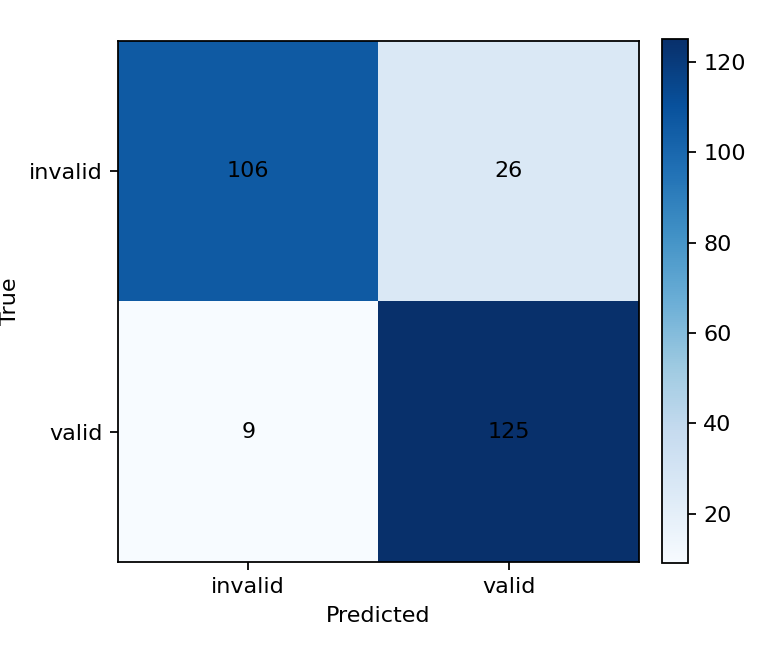
\includegraphics[width=0.78\linewidth]{reports/deep_mobilenet_v3_large/confusion_matrix.png}
\caption{MobileNetV3-Large confusion matrix on the held-out test set.}
\label{fig:cm}
\end{figure}

\begin{figure}[t]
\centering
\begin{minipage}{0.48\linewidth}
\centering
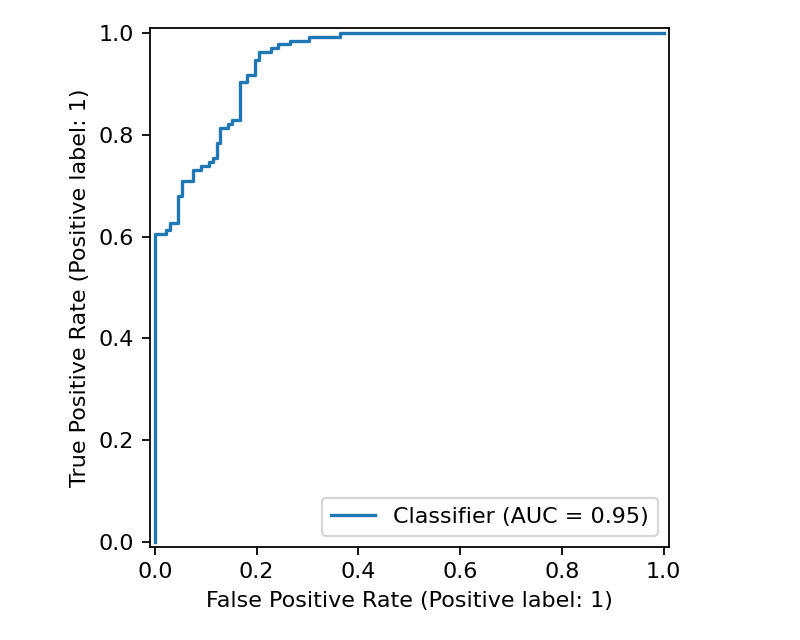
\includegraphics[width=\linewidth]{reports/deep_mobilenet_v3_large/roc_curve.png}
\end{minipage}
\hfill
\begin{minipage}{0.48\linewidth}
\centering
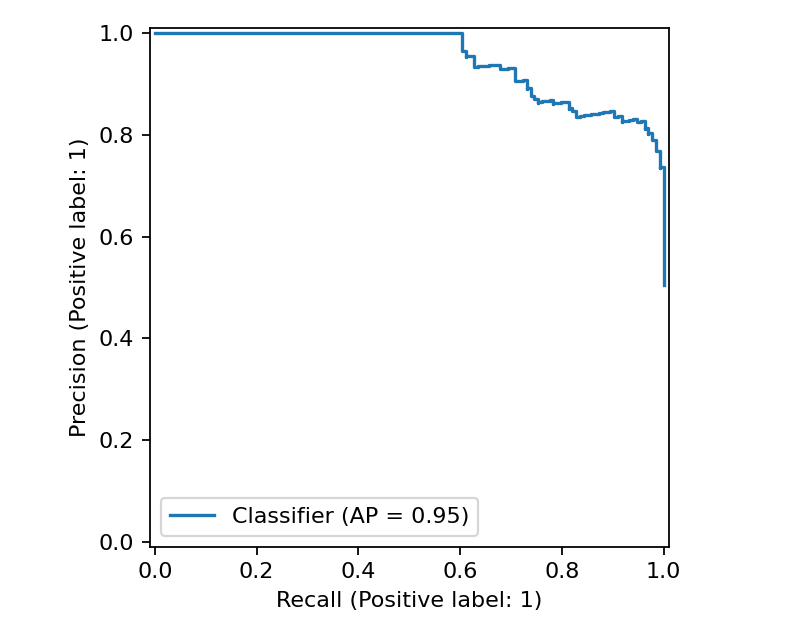
\includegraphics[width=\linewidth]{reports/deep_mobilenet_v3_large/pr_curve.png}
\end{minipage}
\caption{ROC and precision-recall curves for the selected MobileNetV3-Large
model.}
\label{fig:curves}
\end{figure}

\subsection{Model Size}

The saved checkpoints are small enough for a lightweight filtering component.
The MobileNetV3-Large checkpoint is 16.23 MB and the EfficientNet-B0 checkpoint
is 15.57 MB. A latency benchmarking script is included in the repository and is
intended to be run on the target deployment machine. The final model selection
in this report is based on held-out quality metrics and false-negative count.

\section{Error Analysis}

The visual error grids show that many remaining mistakes are plausible hard
cases rather than random failures.

False negatives are mostly valid wheels that are difficult to recognize:
\begin{itemize}
    \item small or low-resolution wheel crops;
    \item dark or blurred wheels;
    \item wheels partially occluded by body parts, mudguards, or image borders;
    \item crops with unusual viewpoint or poor localization.
\end{itemize}

False positives are often invalid crops that still contain strong wheel-like
visual evidence:
\begin{itemize}
    \item partial wheels or tire fragments marked as invalid;
    \item circular rim-like structures;
    \item vehicle parts near the wheel region;
    \item ambiguous crops where the label boundary is not visually obvious.
\end{itemize}

\begin{figure*}[t]
\centering
\begin{minipage}{0.49\textwidth}
\centering
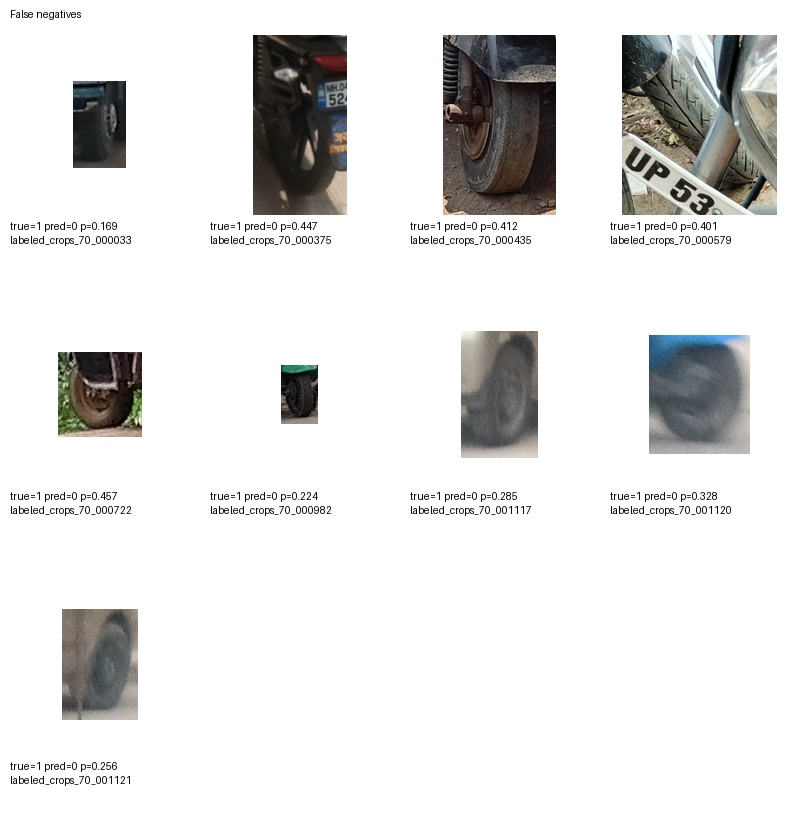
\includegraphics[width=\linewidth]{reports/deep_mobilenet_v3_large/false_negatives.jpg}
\end{minipage}
\hfill
\begin{minipage}{0.49\textwidth}
\centering
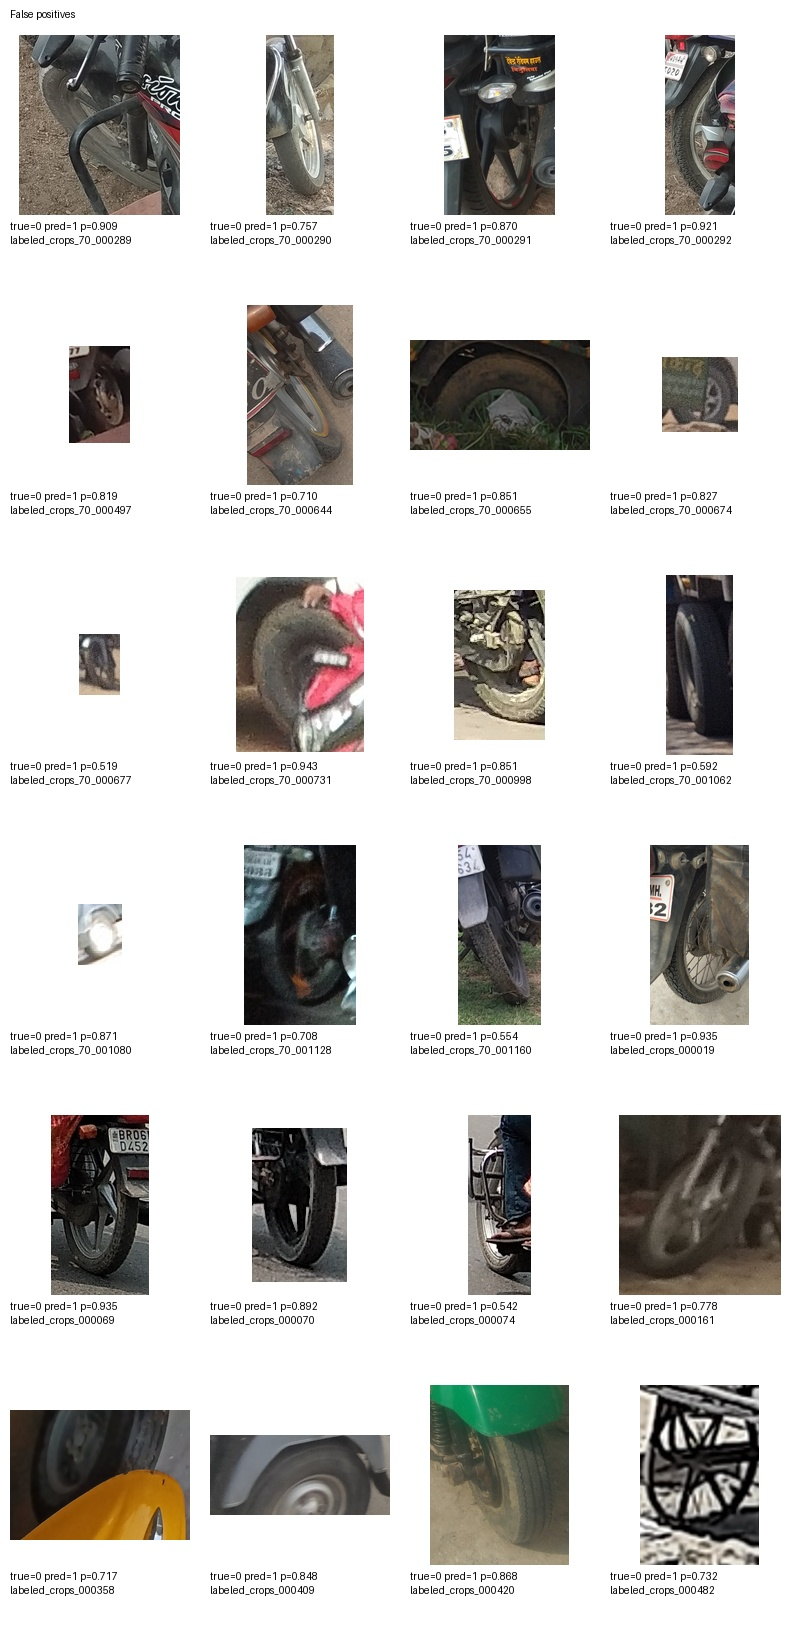
\includegraphics[width=\linewidth]{reports/deep_mobilenet_v3_large/false_positives.jpg}
\end{minipage}
\caption{Examples of MobileNetV3-Large false negatives (left) and false
positives (right). Many errors correspond to visually difficult or semantically
ambiguous crops.}
\label{fig:errors}
\end{figure*}

This error pattern suggests that future improvements should first focus on data
quality: relabeling high-confidence errors, collecting more hard negatives, and
adding more difficult but valid positive examples. A larger model may help in
some cases, but the current results indicate that label ambiguity and limited
hard-case coverage are more important bottlenecks.

\section{Limitations}

The most important limitation is task scope. The model cannot find wheels in a
full vehicle image by itself. It only classifies candidate crops. A full
end-to-end product would need an object detector, region proposal method, or
another candidate-generation stage before this classifier.

The dataset is clean but still modest in size. The held-out test set contains
266 samples from 88 source images, which is suitable for a course project and a
focused prototype, but not enough to claim production-level reliability. A
larger external holdout set with more vehicle types, lighting conditions, and
candidate-generation failure modes would be needed before deployment.

Finally, the model was selected using one fixed split. Multiple random grouped
splits or cross-validation would provide a more stable estimate of variance.
This was left as future work because the main objective was to implement the
complete candidate-filtering pipeline and evaluate it on a leakage-safe held-out
test set.

\section{Conclusion}

The implemented system follows the original project scope: it provides a
reproducible dataset pipeline, a baseline, compact transfer-learning models,
validation-based threshold tuning, held-out test evaluation, and visual error
analysis for wheel-candidate crop filtering.

The selected MobileNetV3-Large model reaches 0.877 valid-class F1 and 0.933
valid-class recall on the test set, while reducing false negatives from 32 for
the baseline to 9. These results support the use of the model as a lightweight
first-stage candidate filter before more expensive virtual wheel try-on
components. The most useful next steps are to improve ambiguous labels, collect
more hard positives and hard negatives, measure latency on target hardware, and
evaluate on a larger external holdout set.

\begin{thebibliography}{99}

\bibitem{mobilenetv3}
A. Howard, M. Sandler, G. Chu, L.-C. Chen, B. Chen, M. Tan, W. Wang,
Y. Zhu, R. Pang, V. Vasudevan, Q. V. Le, and H. Adam,
``Searching for MobileNetV3,'' in \emph{Proc. IEEE/CVF International
Conference on Computer Vision}, 2019.

\bibitem{efficientnet}
M. Tan and Q. V. Le, ``EfficientNet: Rethinking model scaling for
convolutional neural networks,'' in \emph{Proc. International Conference on
Machine Learning}, 2019.

\bibitem{imagenet}
J. Deng, W. Dong, R. Socher, L.-J. Li, K. Li, and L. Fei-Fei,
``ImageNet: A large-scale hierarchical image database,'' in \emph{Proc. IEEE
Conference on Computer Vision and Pattern Recognition}, 2009.

\bibitem{adamw}
I. Loshchilov and F. Hutter, ``Decoupled weight decay regularization,'' in
\emph{Proc. International Conference on Learning Representations}, 2019.

\bibitem{sklearn}
F. Pedregosa et al., ``Scikit-learn: Machine learning in Python,''
\emph{Journal of Machine Learning Research}, vol. 12, pp. 2825--2830, 2011.

\end{thebibliography}

\end{document}
